\section{RTC::Component\-Action Interface Reference}
\label{interfaceRTC_1_1ComponentAction}\index{RTC::ComponentAction@{RTC::ComponentAction}}
Lightweight\-RTC::Conponent\-Action interface.  


{\tt import \char`\"{}RTC.idl\char`\"{};}

Inheritance diagram for RTC::Component\-Action::\begin{figure}[H]
\begin{center}
\leavevmode
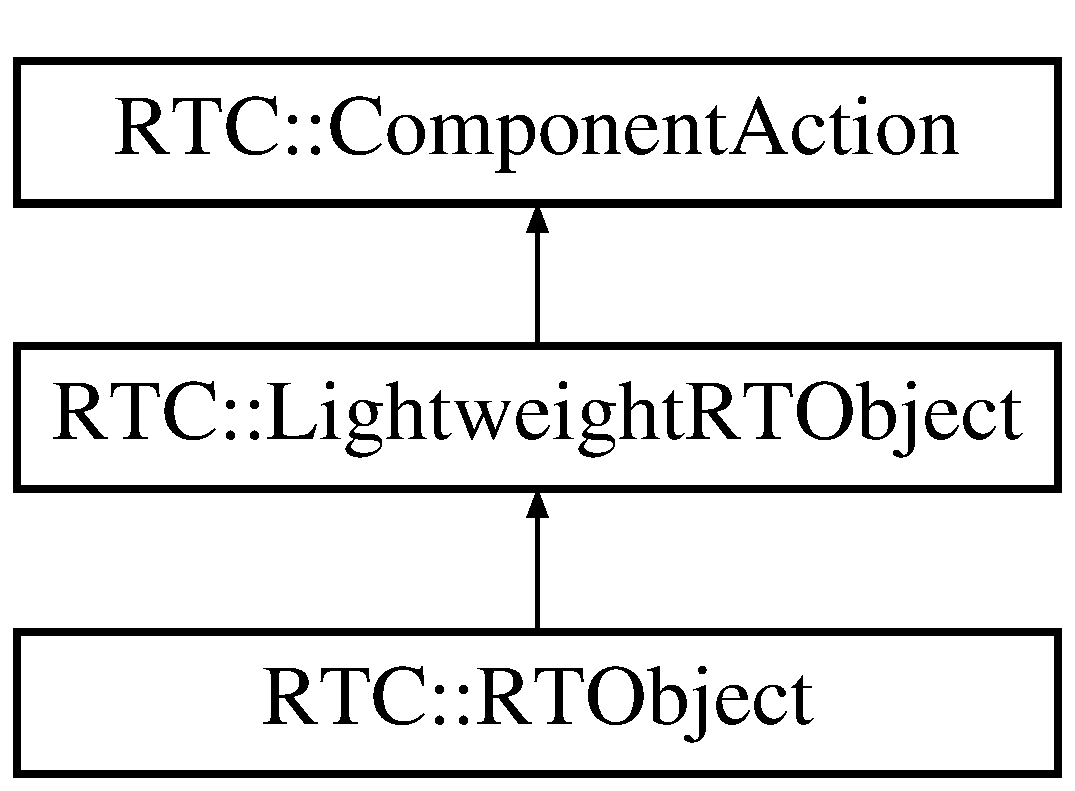
\includegraphics[height=3cm]{interfaceRTC_1_1ComponentAction}
\end{center}
\end{figure}
\subsection*{Public Member Functions}
\begin{CompactItemize}
\item 
{\bf Unique\-Id} {\bf attach\_\-executioncontext} (in {\bf Execution\-Context} exec\_\-context)
\item 
{\bf Return\-Code\_\-t} {\bf detach\_\-executioncontext} (in {\bf Unique\-Id} ec\_\-id)
\item 
{\bf Return\-Code\_\-t} {\bf on\_\-initialize} ()
\item 
{\bf Return\-Code\_\-t} {\bf on\_\-finalize} ()
\item 
{\bf Return\-Code\_\-t} {\bf on\_\-startup} (in {\bf Unique\-Id} ec\_\-id)
\item 
{\bf Return\-Code\_\-t} {\bf on\_\-shutdown} (in {\bf Unique\-Id} ec\_\-id)
\item 
{\bf Return\-Code\_\-t} {\bf on\_\-activated} (in {\bf Unique\-Id} ec\_\-id)
\item 
{\bf Return\-Code\_\-t} {\bf on\_\-deactivated} (in {\bf Unique\-Id} ec\_\-id)
\item 
{\bf Return\-Code\_\-t} {\bf on\_\-aborting} (in {\bf Unique\-Id} ec\_\-id)
\item 
{\bf Return\-Code\_\-t} {\bf on\_\-error} (in {\bf Unique\-Id} ec\_\-id)
\item 
{\bf Return\-Code\_\-t} {\bf on\_\-reset} (in {\bf Unique\-Id} ec\_\-id)
\end{CompactItemize}


\subsection{Detailed Description}
Lightweight\-RTC::Conponent\-Action interface. 



\subsection{Member Function Documentation}
\index{RTC::ComponentAction@{RTC::Component\-Action}!attach_executioncontext@{attach\_\-executioncontext}}
\index{attach_executioncontext@{attach\_\-executioncontext}!RTC::ComponentAction@{RTC::Component\-Action}}
\subsubsection{\setlength{\rightskip}{0pt plus 5cm}{\bf Unique\-Id} RTC::Component\-Action::attach\_\-executioncontext (in {\bf Execution\-Context} {\em exec\_\-context})}\label{interfaceRTC_1_1ComponentAction_RTC_1_1RTObjecta9}


\index{RTC::ComponentAction@{RTC::Component\-Action}!detach_executioncontext@{detach\_\-executioncontext}}
\index{detach_executioncontext@{detach\_\-executioncontext}!RTC::ComponentAction@{RTC::Component\-Action}}
\subsubsection{\setlength{\rightskip}{0pt plus 5cm}{\bf Return\-Code\_\-t} RTC::Component\-Action::detach\_\-executioncontext (in {\bf Unique\-Id} {\em ec\_\-id})}\label{interfaceRTC_1_1ComponentAction_RTC_1_1RTObjecta10}


\index{RTC::ComponentAction@{RTC::Component\-Action}!on_aborting@{on\_\-aborting}}
\index{on_aborting@{on\_\-aborting}!RTC::ComponentAction@{RTC::Component\-Action}}
\subsubsection{\setlength{\rightskip}{0pt plus 5cm}{\bf Return\-Code\_\-t} RTC::Component\-Action::on\_\-aborting (in {\bf Unique\-Id} {\em ec\_\-id})}\label{interfaceRTC_1_1ComponentAction_RTC_1_1RTObjecta17}


\index{RTC::ComponentAction@{RTC::Component\-Action}!on_activated@{on\_\-activated}}
\index{on_activated@{on\_\-activated}!RTC::ComponentAction@{RTC::Component\-Action}}
\subsubsection{\setlength{\rightskip}{0pt plus 5cm}{\bf Return\-Code\_\-t} RTC::Component\-Action::on\_\-activated (in {\bf Unique\-Id} {\em ec\_\-id})}\label{interfaceRTC_1_1ComponentAction_RTC_1_1RTObjecta15}


\index{RTC::ComponentAction@{RTC::Component\-Action}!on_deactivated@{on\_\-deactivated}}
\index{on_deactivated@{on\_\-deactivated}!RTC::ComponentAction@{RTC::Component\-Action}}
\subsubsection{\setlength{\rightskip}{0pt plus 5cm}{\bf Return\-Code\_\-t} RTC::Component\-Action::on\_\-deactivated (in {\bf Unique\-Id} {\em ec\_\-id})}\label{interfaceRTC_1_1ComponentAction_RTC_1_1RTObjecta16}


\index{RTC::ComponentAction@{RTC::Component\-Action}!on_error@{on\_\-error}}
\index{on_error@{on\_\-error}!RTC::ComponentAction@{RTC::Component\-Action}}
\subsubsection{\setlength{\rightskip}{0pt plus 5cm}{\bf Return\-Code\_\-t} RTC::Component\-Action::on\_\-error (in {\bf Unique\-Id} {\em ec\_\-id})}\label{interfaceRTC_1_1ComponentAction_RTC_1_1RTObjecta18}


\index{RTC::ComponentAction@{RTC::Component\-Action}!on_finalize@{on\_\-finalize}}
\index{on_finalize@{on\_\-finalize}!RTC::ComponentAction@{RTC::Component\-Action}}
\subsubsection{\setlength{\rightskip}{0pt plus 5cm}{\bf Return\-Code\_\-t} RTC::Component\-Action::on\_\-finalize ()}\label{interfaceRTC_1_1ComponentAction_RTC_1_1RTObjecta12}


\index{RTC::ComponentAction@{RTC::Component\-Action}!on_initialize@{on\_\-initialize}}
\index{on_initialize@{on\_\-initialize}!RTC::ComponentAction@{RTC::Component\-Action}}
\subsubsection{\setlength{\rightskip}{0pt plus 5cm}{\bf Return\-Code\_\-t} RTC::Component\-Action::on\_\-initialize ()}\label{interfaceRTC_1_1ComponentAction_RTC_1_1RTObjecta11}


\index{RTC::ComponentAction@{RTC::Component\-Action}!on_reset@{on\_\-reset}}
\index{on_reset@{on\_\-reset}!RTC::ComponentAction@{RTC::Component\-Action}}
\subsubsection{\setlength{\rightskip}{0pt plus 5cm}{\bf Return\-Code\_\-t} RTC::Component\-Action::on\_\-reset (in {\bf Unique\-Id} {\em ec\_\-id})}\label{interfaceRTC_1_1ComponentAction_RTC_1_1RTObjecta19}


\index{RTC::ComponentAction@{RTC::Component\-Action}!on_shutdown@{on\_\-shutdown}}
\index{on_shutdown@{on\_\-shutdown}!RTC::ComponentAction@{RTC::Component\-Action}}
\subsubsection{\setlength{\rightskip}{0pt plus 5cm}{\bf Return\-Code\_\-t} RTC::Component\-Action::on\_\-shutdown (in {\bf Unique\-Id} {\em ec\_\-id})}\label{interfaceRTC_1_1ComponentAction_RTC_1_1RTObjecta14}


\index{RTC::ComponentAction@{RTC::Component\-Action}!on_startup@{on\_\-startup}}
\index{on_startup@{on\_\-startup}!RTC::ComponentAction@{RTC::Component\-Action}}
\subsubsection{\setlength{\rightskip}{0pt plus 5cm}{\bf Return\-Code\_\-t} RTC::Component\-Action::on\_\-startup (in {\bf Unique\-Id} {\em ec\_\-id})}\label{interfaceRTC_1_1ComponentAction_RTC_1_1RTObjecta13}




The documentation for this interface was generated from the following file:\begin{CompactItemize}
\item 
{\bf RTC.idl}\end{CompactItemize}
